\section{Adquisición}
\label{sec:adquisicion}

De las tres partes principales que componen el proyecto, ésta es la única en la que el desarrollador no ha tenido opción de decisión. Debido a su voluntad de presentarlo como trabajo monográfico para una asignatura, se ha visto en la obligación de adecuarlo para poder relacionarlo con ésta. Por ello, se ha optado por el desarrollo de la interfaz de usuario y la gestión del envío a través de \textit{LabVIEW}\cite{labview}, software desarrollado por \textit{National Instruments}\cite{ni} y centrado en la instrumentación electrónica.

Sin duda, y como podrá comprobarse a continuación, el consumo de recursos derivado de la adopción de esta solución resulta excesivo para la aplicación deseada. Si bien se trata de un software con gran utilidad en otros ámbitos, en éste en concreto y siempre bajo el punto de vista del autor, su uso podría definirse con la expresión ``matar moscas a cañonazos''. La extensa lista de herramientas, tanto gratuitas como libres y además multiplataforma, que podrían haberse utilizado resulta difícil de reproducir. Por poner algunos ejemplos, podrían mencionarse las bibliotecas GTK+\cite{gtk} y Qt\cite{qt}, en conjunto con cualquiera de los muchos lenguajes de programación que las soportan (C++, Java, Ruby, D, Perl, Python, PHP...). Como ya se expondrá en la sección \ref{sec:transmision}, correspondiente a la transmisión, la interfaz y protocolo utilizados están ampliamente extendidos y se dispone de librerías en prácticamente la totalidad de los lenguajes.

Tras esta introducción, se presenta la aplicación en sí, creada como un VI y posteriormente empaquetada en un ejecutable, que finalmente se ha utilizado para la generación de un instalador. Se perciben dos partes muy diferenciadas\footnote{El diagrama completo se encuentra en el \hyperref[anexoa]{Anexo A}} en ésta y así se presentarán: por un lado la aplicación base (aquella encargada de adquirir y enviar los datos) y por otra todos los aspectos estéticos que contribuyen a la apariencia del programa pero resultan inútiles desde un punto de vista operativo.

\subsection{Aplicación base}

La base de esta parte del proyecto es la adquisición de datos y el envío de éstos a través de la interfaz seleccionada. Como puede verse en la figura \ref{fig:acher_visa}, todo ello se consigue mediante tres bloques específicamente desarrollados para transmitir cadenas de caracteres a través del puerto de serie. El primero de ellos, obtenido con el nombre \textit{VISA Configure Serial Port} en el grupo \textit{VISA} dentro del apartado \textit{Instrument I/O} de la paleta de funciones, recibe los parámetros de configuración para definir el funcionamiento del protocolo, que más adelante se tratará en el apartado \ref{subsec:trama}.

\begin{figure}[!htp]
\centering
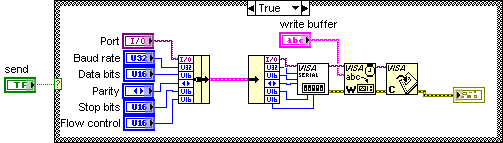
\includegraphics[width=300pt]{./images/acher_visa.png}
\caption{Envío de datos con \textit{LabVIEW}.}
\label{fig:acher_visa}
\end{figure}

Con el objetivo de hacer la aplicación lo más versátil posible, dentro de las limitaciones que su naturaleza establece, se han creado controladores para que el usuario tenga la posibilidad de configurar el tipo de comunicación, aunque están fijados por defecto los valores utilizados en este proyecto.

Para mejorar la legibilidad del código, se han unido todas las señales de los controladores en un cluster que después se ha separado a la entrada del bloque. En este caso en concreto, no supone una gran ventaja, pero es un avance de cara a futuras modificaciones.

El segundo bloque, \textit{VISA Write}, recibe como parámetro el string a enviar. Tal como se ha diseñado, envía los caracteres del string uno a uno, de forma secuencial y una sola vez. El bloque permite la especificación de un pequeño retardo entre caracteres. Se han realizado pruebas y se ha constatado que para la aplicación que se ha desarrollado no es necesaria la inclusión de dicha funcionalidad. El string a enviar se ha definido como un controlador, pues el objetivo es que el usuario final pueda decidir qué mostrar en la matriz de LEDs, y no que se envíe siempre el mismo contenido.

El último de los bloques, \textit{VISA Close}, cierra y termina la comunicación. La figura \ref{fig:acher_visa} muestra cómo se ha pasado el apuntador que indica el puerto a utilizar de un bloque a otro. Lo mismo se ha hecho con el cluster de error. Que finalmente enlaza con un \textit{Simple Error Handler}, para que el usuario pueda tener constancia e información cuando suceda algún error en la comunicación.

\subsection{Apariencia}

\subsubsection{Interfaz}

Una vez definida la funcionalidad base de la aplicación y para mejorar la apariencia de ésta, haciendo más fácil y visual su uso, se han realizado múltiples modificaciones mediante el uso de \textit{Property nodes} principalmente, aunque también se han utilizado otros recursos.

Se ha creado un indicador personalizado\cite{customcontrol} para mostrar una imagen en formato PNG con transparencia. Esta imagen corresponde al logotipo del proyecto que puede verse en la figura \ref{fig:acher_front}. No es ésta la forma más elegante de mostrar una imagen estática, pues para eso se dispone de otros recursos específicos, pero ha resultado la más fácil y rápida desde el punto de vista del desarrollador. Se ha modificado un indicador de tipo booleano para que muestre la misma imagen independientemente del valor que se le asigne. Este indicador puede encontrarse con el nombre \textit{logo\_acher.ctl} entre las fuentes del proyecto.

El controlador de tipo string que define el contenido a enviar por la aplicación se ha configurado mediante \textit{Property nodes} para que el texto aparezca siempre centrado y el tamaño sea mayor que el que aparece por defecto. Estos parámetros son constantes, por lo que el usuario no puede modificarlos durante la ejecución.

\begin{figure}[!htp]
\centering
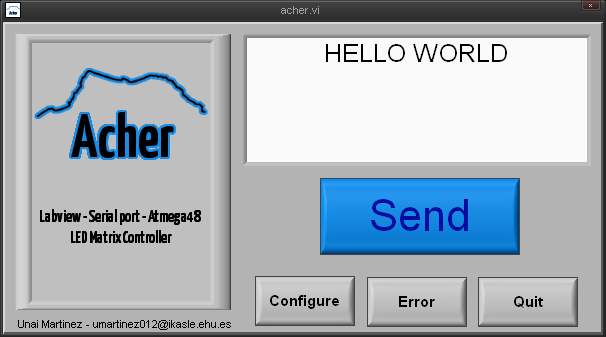
\includegraphics[width=300pt]{./images/acher_front.png}
\caption{Panel frontal: vista general.}
\label{fig:acher_front}
\end{figure}

Se han creado cuatro botones (controladores booleanos) para que el usuario pueda interactuar con la aplicación. Éstos son \textit{Send}, \textit{Configure}, \textit{Error} y \textit{Quit}.

\begin{itemize}

\item{\textbf{Send}:

La función de este botón es enviar, al pulsar sobre él, el contenido del controlador de tipo string:

Todo el programa se encuentra dentro de un bucle \textit{while}. El valor del botón \textit{Send} controla una estructura \textit{case} dentro del \textit{while}. Cuando es verdadera, se ejecuta la aplicación base analizada en la sección anterior. Mientras sea falsa, no se ejecuta acción ninguna.

Mediante los \textit{Property nodes} se han modificado el tamaño y color del texto y el color de fondo del botón. Este último, además, cambia cuando el botón está pulsado. El texto se encuentra en todo momento centrado tanto vertical como horizontalmente.
}

\item{\textbf{Configure}:

Este botón muestra y oculta los controladores que definen los parámetros a utilizar por el bloque \textit{VISA Configure Serial Port}. Para ello, actúa sobre la propiedad de visibilidad de éstos, además de sobre la misma propiedad del indicador utilizado para mostrar el logotipo y el \textit{Simple Error Handler}. También afecta al parámetro \textit{Disabled} del controlador string, del botón \textit{Send} y del botón \textit{Error}.

\begin{figure}[!htp]
\centering
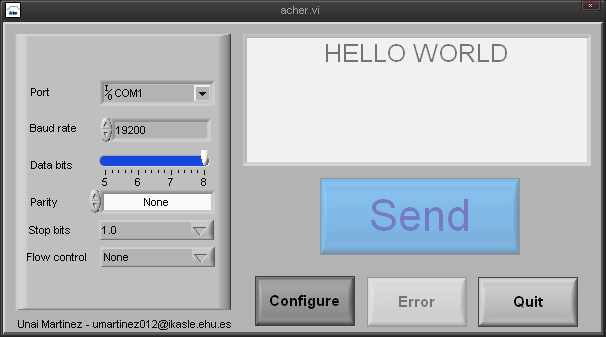
\includegraphics[width=275pt]{./images/acher_config.png}
\caption{Panel frontal: configure.}
\label{fig:acher_config}
\end{figure}

De esta manera, cuando el botón se encuentra pulsado y por lo tanto su valor es verdadero (Figura \ref{fig:acher_config}), se muestran únicamente los controladores de configuración, deshabilitando el controlador string y los botones \textit{Send} y \textit{Error}. El logo y el gestor de error se ocultan. Una vez el usuario ha realizado las modificaciones oportunas, la desactivación del botón \textit{Configure} devuelve la aplicación al estado mostrado en la vista general (Figura \ref{fig:acher_front}).

El tamaño del texto del botón y su alineación tanto horizontal como vertical se encuentran definidas mediante constantes.
}

\item{\textbf{Error}:

\begin{figure}[!htp]
\centering
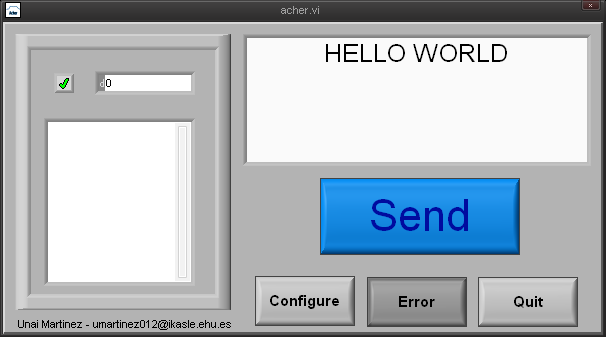
\includegraphics[width=275pt]{./images/acher_err1.png}
\caption{Panel frontal: no error.}
\label{fig:acher_err1}
\end{figure}

El funcionamiento de este botón, muy parecido al de \textit{Configure}, simplemente oculta el logo y muestra el gestor de errores cuando se encuentra pulsado (Figura \ref{fig:acher_err1}). Se debe tener en cuenta que \textit{Configure} tiene prioridad sobre \textit{Error}, por lo que el primero deberá estar desactivado para poder ver el gestor de errores.

El tamaño del texto del botón y su alineación tanto horizontal como vertical se encuentran definidas mediante constantes y mantienen su valor durante toda la ejecución. No así el color de fondo. Cuando se detecta algún error en el envío, éste cambia a rojo (Figura \ref{fig:acher_err2}), indicando así que no se ha efectuado correctamente.

\begin{figure}[!htp]
\centering
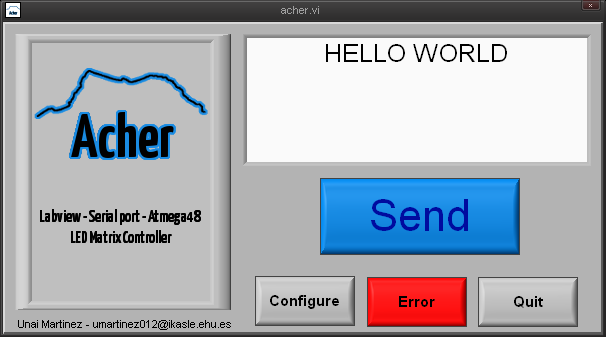
\includegraphics[width=275pt]{./images/acher_err2.png}
\caption{Panel frontal: error.}
\label{fig:acher_err2}
\end{figure}

Pulsando sobre el botón, se puede ver cuál es el error (Figura \ref{fig:acher_err3}). Para diferenciar cuándo se encuentra pulsado y cuándo no, en la nueva definición de color se han especificado dos constantes diferentes, siendo el segundo ligeramente más oscuro. Un simple \textit{select} controlado por el estado del botón booleando \textit{Error} decide cuál utilizar.

\begin{figure}[!htp]
\centering
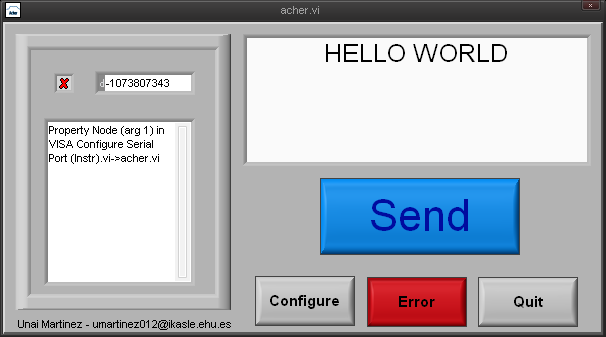
\includegraphics[width=275pt]{./images/acher_err3.png}
\caption{Panel frontal: view error.}
\label{fig:acher_err3}
\end{figure}
}

Al realizar un nuevo envío correcto, y por lo tanto no haber ningún error en el gestor de errores, el botón adquiere de nuevo el color original.

\item{\textbf{Quit}:

Para evitar que el usuario salga de la aplicación por error, la pulsación del botón \textit{Quit} controla una estructura \textit{case}. Cuando el valor es falso, éste se pasa directamente al controlador que termina el bucle \textit{while}, permitiendo que la aplicación siga ejecutándose. Cuando es verdadero, se lanza una ventana que pide confirmación al usuario (Figura \ref{fig:acher_quit}).

\begin{figure}[!htp]
\centering
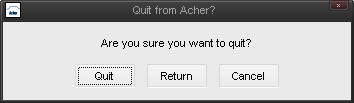
\includegraphics[width=175pt]{./images/acher_quit.png}
\caption{Ventana de salida.}
\label{fig:acher_quit}
\end{figure}

El lanzamiento de esta ventana se efectúa mediante el bloque \textit{Three Button Dialog}. Éste recibe como parámetros el contenido de los tres botones, el título de la ventana, el texto a mostrar y la alineación (Figura \ref{fig:acher_quitcase}). Un bloque de comparación hace que la salida sólo sea verdadera cuando el usuario pulse sobre el botón de la izquierda (\textit{Quit}). Cualquiera de las otras opciones (\textit{Return} o \textit{Cancel}), devolverá una salida falsa, permitiendo que se siga ejecutando el bucle principal.

\begin{figure}[!htp]
\centering
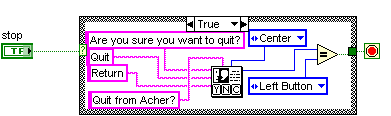
\includegraphics[width=225pt]{./images/acher_quitcase.png}
\caption{Lógica de salida.}
\label{fig:acher_quitcase}
\end{figure}
}

\end{itemize}

\subsubsection{Icono, patrón y ventana}

El icono y el patrón del VI se han personalizado para adecuarlos al proyecto. El icono reproduce el logotipo\footnote{El icono está disponible en las fuentes con el nombre \textit{acher\_icon.ico}}, mientas el patrón indica que no hay ninguna salida ni entrada, pues se trata de un VI que trabaja de forma autónoma.

Por otra parte, en las propiedades del VI se ha configurado como de tipo \textit{ventana de diálogo} para que no aparezcan los controles propios de \textit{LabVIEW} durante a ejecución. Además, el tamaño de ésta se ha adecuado al del panel frontal.

\subsection{Ejecutable e instalador}

Con el fin de facilitar el uso de la aplicación y para favorecer su portabilidad (entre equipos, no entre plataformas), se ha creado un ejecutable a partir del VI desarrollado. Para realizar este proceso, simplemente se ha creado un proyecto\footnote{El fichero del proyecto está disponible en las fuentes con el nombre \textit{acher.lvproj}} y, tras realizar las selecciones pertinentes (icono, nombres, rutas, etc.), se ha construido mediante el \textit{Application Builder} del propio \textit{LabVIEW}. Una vez obtenido el ejecutable, y haciendo uso de la misma herramienta\cite{installer}, se ha construido un instalador. En éste, además del ejecutable, el icono y otras opciones de personalización, se han añadido \textit{NI LabVIEW Run-Time Engine 2009} y \textit{NI-VISA Runtime 4.5}, un conjunto de librerías y drivers que permiten la instalación y ejecución del programa en aquellos equipos donde no esté instalado \textit{LabVIEW}.

El resultado final es un instalador de aproximadamente 150MB que nos garantiza la posibilidad de ejecutar el programa en cualquier equipo con un sistema operativo compatible y un puerto serie. Las condiciones de distribución y utilización se rigen por la licencia de \textit{LabVIEW}, pues es el software sobre el que corre la aplicación.

\subsubsection{Cierre del VI}

\begin{figure}[!htp]
\centering
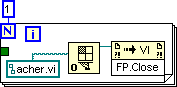
\includegraphics[width=150pt]{./images/acher_close.png}
\caption{Lógica de cierre del VI.}
\label{fig:acher_close}
\end{figure}

Debido a las características de ejecución de \textit{LabVIEW}, una vez terminado el bucle \textit{while}, es decir, cuando el usuario haya pulsado el botón \textit{Quit} y confirmado la acción en la ventana emergente, el VI se mantiene abierto, aunque parado. Aunque ésta es una característica muy útil (prácticamente imprescindible) en el proceso de desarrollo, resulta inadecuada en la aplicación final. Por un lado porque el usuario se ve obligado a cerrar una ventana más, a pesar de haber solicitado y confirmado el cierre de la aplicación. Por otro, porque una vez ha terminado la ejecución, e independientemente del tipo de configuración que se haya seleccionado en las propiedades del VI, se muestran menús propios de \textit{LabVIEW}. Éstos pueden producir confusión en el usuario, al desconocer su funcionalidad y la razón por la que aparecen. Además, en principio, no es de su interés el software utilizado para el desarrollo de la aplicación.

Para forzar el cierre del VI\cite{closevi} una vez se ha confirmado por parte del usuario, se ha añadido un bucle \textit{for} de una sola iteración (que actúa como un \textit{frame} secuencial) a continuación del \textit{while} principal (Figura \ref{fig:acher_close}). Dentro de éste encontramos un bloque del tipo \textit{Open VI Reference} al que se pasa como argumento el nombre del propio VI y un bloque \textit{Invoke Node} con el método \textit{Close FP} seleccionado que recibe el apuntador creado por el anterior.